\documentclass[10pt,a4paper,onecolumn]{article}

\usepackage[utf8]{inputenx}
\usepackage[T1]{fontenc}
\usepackage{lmodern}
\usepackage{listings}
\usepackage{textcomp}
\usepackage[english,italian]{babel}
\usepackage{amsmath}
\usepackage{booktabs}
\usepackage{graphicx}
\usepackage[font=small,labelfont=bf,labelsep=period,tableposition=top]{caption}
\usepackage{tabularx}
\usepackage{multirow}
\usepackage{longtable}
\usepackage{fancyhdr}
\usepackage{lastpage}
\usepackage{color}
\usepackage{enumitem}
\usepackage{float}


\fancyhead{}
\renewcommand{\headrulewidth}{1pt}

\fancyhead[RE,RO]{
\begin{picture}(-135,0)
	\put(-475,0){\sffamily\large\leftmark}
\end{picture}
}

\cfoot{}

\fancyfoot[RO,LE]{\sffamily Pag.~\thepage{} di \pageref{LastPage}}
\fancyfoot[RE,LO]{MUI - Museo Universitario Italiano}

\renewcommand{\footrulewidth}{.2pt}
\pagestyle{fancy}

\renewcommand{\sectionmark}[1]{\markboth{#1}{#1}}

% **************************************************
% Cross-references e collegamenti ipertestuali
% **************************************************
%\usepackage[bookmarks=true,hyperfootnotes=false,hidelinks,colorlinks=true, pdfnewwindow]{hyperref}
\usepackage{hyperref}

%\usepackage[hidelinks]{hyperref}
\hypersetup{%
  colorlinks=false, hidelinks=true, linktocpage=false, pdfborder={0,0,0}, pdfstartpage=1, pdfstartview=FitV,%
  urlcolor=Cyan, linkcolor=Cyan, citecolor=Black, %pagecolor=Black,
  pdfcreator={pdflatex}, pdfproducer={pdflatex with hyperref package}%
}

\definecolor{dkgreen}{rgb}{0,0.6,0}
\definecolor{gray}{rgb}{0.5,0.5,0.5}
\definecolor{mauve}{rgb}{0.58,0,0.82}

\lstset{ %
  %language=XHTML,                % the language of the code
  basicstyle=\footnotesize,           % the size of the fonts that are used for the code
  numbers=left,                   % where to put the line-numbers
  numberstyle=\tiny\color{gray},  % the style that is used for the line-numbers
  stepnumber=2,                   % the step between two line-numbers. If it's 1, each line
                                  % will be numbered
  numbersep=5pt,                  % how far the line-numbers are from the code
  backgroundcolor=\color{white},      % choose the background color. You must add \usepackage{color}
  showspaces=false,               % show spaces adding particular underscores
  showstringspaces=false,         % underline spaces within strings
  showtabs=false,                 % show tabs within strings adding particular underscores
  frame=single,                   % adds a frame around the code
  rulecolor=\color{black},        % if not set, the frame-color may be changed on line-breaks within not-black text (e.g. comments (green here))
  tabsize=2,                      % sets default tabsize to 2 spaces
  captionpos=b,                   % sets the caption-position to bottom
  breaklines=true,                % sets automatic line breaking
  breakatwhitespace=false,        % sets if automatic breaks should only happen at whitespace
  title=\lstname,                   % show the filename of files included with \lstinputlisting;
                                  % also try caption instead of title
  keywordstyle=\color{blue},          % keyword style
  commentstyle=\color{dkgreen},       % comment style
  stringstyle=\color{mauve},         % string literal style
  escapeinside={\%*}{*)},            % if you want to add LaTeX within your code
  morekeywords={*,...},              % if you want to add more keywords to the set
  deletekeywords={...}              % if you want to delete keywords from the given language
}

% **************************************************
\newcommand{\sitepage}[1]{\textcolor{cyan}{\textsf{#1}}}
\newcommand{\inglese}[1]{\foreignlanguage{english}{\itshape{}#1}}
\newcommand{\progname}[1]{\textcolor{blue}{\textsf{#1}}}



%INIZIO DEL DOCUMENTO=================================================
%=====================================================================
%=====================================================================

\begin{document}
\begin{titlepage}
\begin{center}


\includegraphics[width=0.6\textwidth]{logo_mui.png}\\
\vspace{60pt}
\textsc{\Huge Museo Universitario Italiano}\\
\vspace{30pt}
\textsc{\Large Progetto del corso Tecnologie Web\\ AA 2016/17}\\
\vspace{10pt}
\begin{table}[H]
    \centering
    \begin{tabular}{ r l }
        1099872 & Fabio Vianello\\
        1097458 & Silvio Meneguzzo\\
        1097588 & Giovanni Prete\\
        1093209 & Giulia Petenazzi\\
    \end{tabular}
\end{table}

\vspace{30pt}
\textbf{Indirizzo sito}:\\ \url{http://tecweb2016.studenti.math.unipd.it/gpetenaz/}\\
\vspace{5pt}
\textbf{Utente admin (segreteria)}: admin - admin\\
\textbf{Utente semplice (guida)}: user - user\\
\vspace{10pt}
\textbf{Email referente}:\\ \href{mailto:giovani.prete.1@studenti.unipd.it}{giovani.prete.1@studenti.unipd.it}

\end{center}
\end{titlepage}
%-----------------------------------------------------------------------

\clearpage
\tableofcontents

\clearpage
\section{Abstract}
Questo progetto consiste nella realizzazione di un sito per un ipotetico museo contenente opere d'arte create dagli studenti degli istituti universitari italiani.
Si tratta di un sito possibilmente adattabile per qualsiasi museo di piccole e medie dimensioni.
Offre agli utenti servizi quali:
\begin{itemize}
\item visualizzazione delle informazioni generali del museo;
\item acquisto biglietti (funzionalità non implementata in maniera effettiva ma solo a livello dimostrativo);
\item area amministrazione per la segreteria;
\item area amministrazione per le guide.
\end{itemize}
Il sito è accessibile al maggior numero di utenti possibile.

\clearpage
\section{Analisi dei requisiti}
\subsection{Requisiti essenziali}
Il sito dovrà avere come target tutti i possibili utenti interessati a visitare il museo.
Le informazioni di maggiore interesse devono essere facilmente e velocemente reperibili.
L'utente finale vorrà avere informazioni riguardo il museo, ed eventualmente acquistarne dei biglietti.
L'utente deve poter trovare informazioni riguardo:
\begin{itemize}
 \item la storia e l'intento del museo;
 \item orari in cui si possono effettuare le visite;
 \item i servizi offerti, tra cui:
	 \begin{itemize}
	 \item guardaroba;
	 \item bar;
	 \item pizzeria;
	 \item negozio.
	 \end{itemize}
 \item le tipologie ed i prezzi dei biglietti;
 \item i tour guidati che sono offerti;
 \item i contatti;
 \item la localizzazione geografica del museo.
 \end{itemize}
L'utente deve poter acquistare un set di biglietti per un certo giorno, avendo la possibilità di specificare un nominativo, il tour a cui desidera partecipare, il numero di biglietti per ogni tipologia. Al termine della procedura di acquisto l'utente dovrà visualizzare un messaggio di errore in caso di fallimento dell'acquisto oppure un messaggio di avvenuto acquisto.\\
 Deve essere predisposta un'area amministrazione da cui la segreteria, una volta autenticata, possa:
 \begin{itemize}
 \item visualizzare i biglietti che sono stati venduti in riferimento a un certo periodo di tempo;
 \item aggiungere tours guidati;
 \item visualizzare e modificare i tours già esistenti;
 \item modificare le tipologie di biglietti disponibili.
 \end{itemize}
 Infine deve essere predisposta un'area da cui le guide, una volta autenticate, possano:
 \begin{itemize}
 	\item visualizzare i biglietti che sono stati venduti in riferimento a un certo periodo di tempo;
 	\item visualizzare, modificare tours guidati;
 \end{itemize}

 I colori dominanti saranno rosso scuro e nero, per richiamare i colori all'interno del museo e per dare all'utente la sensazione di trovarsi in un luogo raffinato ed elegante come è il museo.\\
 Le pagine HTML e i file CSS devono validare secondo lo standard W3C.

\subsection{Categorie di utenti}
Il sito è quindi destinato a tre categorie di utenti:
\begin{itemize}
\item utente non loggato, spesso denominato "utente": ha accesso a tutte le pagine tranne quelle di amministrazione;
\item utente loggato come "segreteria":  ha accesso alle pagine di amministrazione, oltre che alle pagine dell'utente non loggato;
\item utente loggato come "guida": ha accesso alle pagine di amministrazione per le guide, oltre che alle pagine dell'utente non loggato.
\end{itemize}

 \subsection{Mappa indicativa del sito}
 \subsubsection{Pagine consultabili dal pubblico}
 Le pagine consultabili dal pubblico sono:
  \begin{itemize}
 	\item home page;
 	\item orari e servizi;
 	\item biglietti;
    \begin{itemize}
 		\item pagina di acquisto biglietti;
    \end{itemize}
 	\item tours;
 	\item contatti;
 	\item dove siamo.
 \end{itemize}
 \subsubsection{Pagina di login}
 Nel footer della home page è presente il link per la pagina di login per la segreteria e per le guide. Se i dati inseriti sono corretti l'accesso è eseguito con successo e verrà mostrato all'utente autenticato la relativa pagina di amministrazione in base alla sua tipologia. Se invece i dati sono errati verrà visualizzato un messaggio di errore e verrà riproposto il form per eseguire il login. L'errore visualizzato non specifica quale dei due campi è sbagliato per evitare di dare informazioni sulla correttezza o meno dello username ad eventuali utenti malintenzionati.
 \subsubsection{Pagine di amministrazione}
 Le pagine di amministrazione accessibili dipendono dalla tipologia di utente, segreteria o guida, e sono le seguenti:
 \begin{itemize}
 \item pagina di avvenuto accesso;
 \item home page di amministrazione, contenente i link per:
    \begin{itemize}
	\item Cerca e visualizza biglietti;
    \item Visualizza e modifica i tour;
	\item Visualizza e modifica le tipologie di biglietti (unicamente per la segreteria);
	\item Aggiungi tour (unicamente per la segreteria);
 	\end{itemize}
 \end{itemize}

\clearpage
\section{Database}
Il database presenta cinque tabelle:
 \begin{itemize}
     \item Utenti;
     \item Tours;
     \item Prezzi;
     \item Biglietti;
     \item AssPrezzi.
 \end{itemize}
Un Utente è caratterizzato da:
\begin{itemize}
    \item nome;
    \item ruolo (a scelta tra segreteria e guide);
    \item username;
    \item password.
\end{itemize}
Un Tour è caratterizzato da;
\begin{itemize}
    \item nome;
    \item breve descrizione;
    \item prezzo in euro;
    \item guida.
\end{itemize}
Un Prezzo è caratterizzato da:
\begin{itemize}
    \item descrizione (ad esempio intero, ridotto, ecc...);
    \item prezzo in euro;
    \item prezzo di noleggio dell'audioguida.
\end{itemize}
Un Biglietto è caratterizzato da:
\begin{itemize}
    \item nominativo;
    \item data della visita;
    \item una lista di prezzi associati al biglietto.
\end{itemize}
Infine la tabella AssPrezzi è caraterizzata dai seguenti campi:
\begin{itemize}
    \item biglietto;
    \item prezzo;
    \item quantità.
\end{itemize}
Un Biglietto può quindi riferirsi a più prezzi contemporaneamente, mentre un prezzo può appartenere a più biglietti contemporaneamente. Si realizza così una relazione N-N tra la tabella Biglietti e la tabella Prezzi, tale relazione viene espressa attraverso la tabella AssPrezzi.\\
Supponiamo ad esempio che Mario voglia acquistare un biglietto intero e due ridotti, mentre Lucia tre interi e quattro ridotti. La tabella AssPrezzi sarà quindi:
\begin{table}[H]
    \centering
    \begin{tabular}{ | c | c | c |}
        \hline
        \textbf{biglietto} & \textbf{prezzo} & \textbf{quantità} \\
        \hline
        id-biglietto-mario & id-prezzo-intero & 1 \\
        \hline
        id-biglietto-mario & id-prezzo-ridotto & 1 \\
        \hline
        id-biglietto-lucia & id-prezzo-intero & 3 \\
        \hline
        id-biglietto-lucia & id-prezzo-ridotto & 4 \\
        \hline
    \end{tabular}
    \caption{Esempio tabella AssPrezzi}
\end{table}

Il prezzo totale deve essere calcolato come somma tra il prezzo dei vari biglietti (dato dalla somma dei vari prezzi associati a quel biglietto) e tra il prezzo del tour eventualmente scelto (dato dal prodotto tra il numero di persone totali del biglietto per il prezzo del tour).
\begin{figure}[h!]
\centering
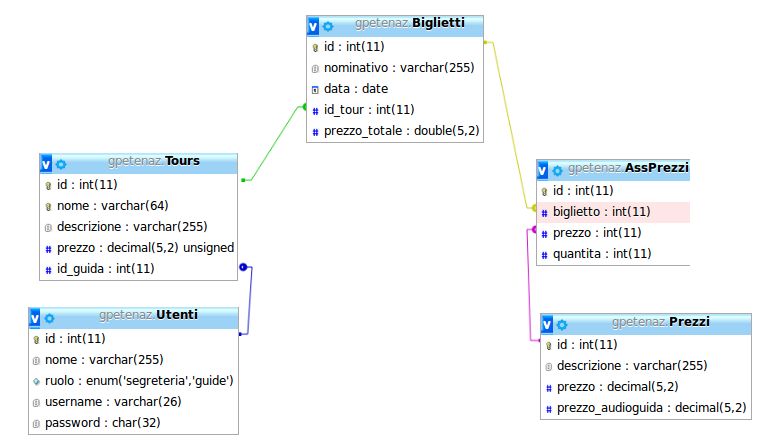
\includegraphics[scale=0.50]{db.png}
\caption{Schema del database}
\end{figure}

\clearpage
\section{Design}
\subsection{Layout}
Sono stati fatti attenti studi e confronti tra i siti di altri musei che hanno portato alla decisione di utilizzare un layout a schede, che risulta molto intuitivo agli occhi degli utenti finali. Lo svantaggio principale di questo tipo di layout, ovvero la poca manutenibilità in caso di espansione del menu, risulta molto limitato dal fatto che difficilmente si dovranno aggiungere molte altre schede. Eventuali espansioni future del museo infatti produrrebbero informazioni da aggiungere a sezioni già esistenti, è quindi poco probabile che ci sia la necessità di aggiungere voci al menù. Allo stato attuale il menu presenta sei schede, e contiene lo spazio per l'aggiunta in caso di sviluppi futuri.\\
All'interno di un pagina del sito possiamo trovare i seguenti elementi:
\begin{itemize}
 \item header: sezione superiore che contiene il titolo della pagina e il logo;
 \item nav: sezione sottostante all'header, contiene il menu di navigazione con i link alle pagine principali;
 \item path: sezione sottostante al nav, contiene la posizione attuale all'interno del sito;
 \item content: contenuto della pagina;
 \item footer: sezione inferiore che contiene le informazioni accessorie come le certificazione W3C. Nella home page viene anche mostrato il link all'area amministrazione.
\end{itemize}
Per garantire una corretta visualizzazione del sito da dispositivi aventi dimensioni di schermo diverse è stato utilizzato un layout elastico.
Per realizzare ciò, per definire le dimensioni degli elementi nel foglio di stile sono state utilizzate le percentuali e/o unità di misura degli em. Gli elementi della pagina vengono quindi dimensionati efficacemente negli schermi più grandi, fino ad arrivare a un punto di rottura che fa cambiare il posizionamento dei vari elementi, in primo luogo dei link del menu di navigazione. Grazie alla completa separazione tra contenuto e presentazione il contenuto in HTML delle pagine non è stato cambiato, mentre si sono scritti diversi file CSS per organizzare la presentazione.
I file CSS scritti sono:
\begin{itemize}
    \item stylesheet.css:  stabilisce la presentazione per gli schermi medio grandi (es: pc desktop e tablet più grandi)
    \item stylesheet\_mobile.css: stabilisce la presentazione per gli schermi piccoli(es: smartphone e tablet più piccoli). Vista la corretta definizione dello stylesheet.css è stato possibile scrivere questo file apportando pochissime modifiche rispetto allo stylesheet.css, aumentando significativamente la qualità della presentazione dei contenuti, specialmente nella pagina di acquisto biglietti.
    \item sylesheet\_print.css: stabilisce la presentazione per la stampa delle pagine del sito.
\end{itemize}
Sono stati utilizzati dei Google font, ma per fornire il supporto adeguato in caso di problemi, sono stati definite famiglie di font aggiuntive "standard".
Per preservare l’accessibilità e la corretta visualizzazione su qualsiasi dispositivo (anche i più datati), le regole CSS3 si sono limitate a funzionalità grafiche di dettaglio poco rilevanti. In particolare sono stati utilizzati i \textit{gradienti}, i \textit{border-radius}, e una piccola transazione nel menu, per rendere più gradevole la navigazione. Qualora CSS3 non fosse disponibile, è sempre garantita la corretta visualizzazione dei contenuti.
\begin{figure}[h]
\centering
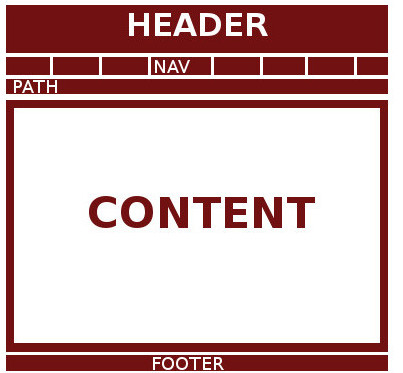
\includegraphics[scale=0.40]{mock_up.jpg}
\caption{Layout da pc desktop}
\end{figure}
\begin{figure}[h]
\centering
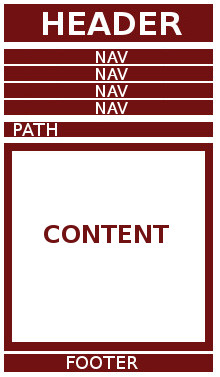
\includegraphics[scale=0.40]{mock_up_mobile.jpg}
\caption{Vista da smartphone}
\end{figure}

\clearpage
\begin{figure}[H]
\centering

\includegraphics[scale=0.35]{vista_desktop.png}
\caption{Layout da pc desktop della home page}
\end{figure}
\begin{figure}[H]
\centering
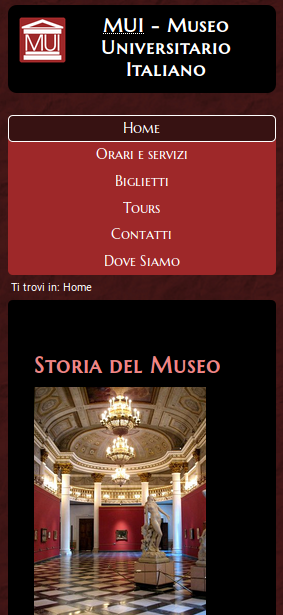
\includegraphics[scale=0.35]{vista_mobile.png}
\caption{Layout da smartphone della home page}
\end{figure}

\begin{figure}[h]
\centering
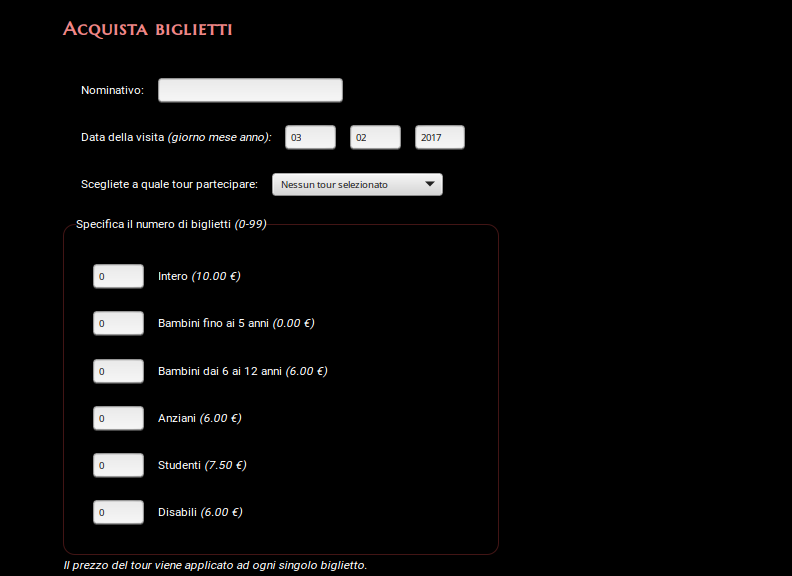
\includegraphics[scale=0.30]{form_desktop.png}
\caption{Vista da pc desktop del form}
\end{figure}
\begin{figure}[h]
\centering
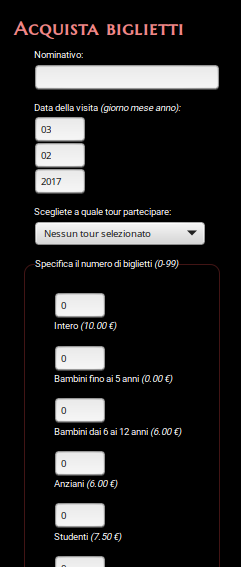
\includegraphics[scale=0.45]{form_mobile.png}
\caption{Vista da smartphone del form}
\end{figure}

\clearpage
\subsection{Organizzazione dei contenuti}
I contenuti sono stati organizzati essenzialmente nelle sei pagine alle quali si può accedere dal menu, in modo da evitare il disorientamento.
Dalla pagina dei Biglietti l'utente può andare alla pagina di acquisto biglietti attraverso un link ben visibile presente nella parte superiore della pagina.
Ogni pagina presenta contenuti ben strutturati, con testi chiari e comprensibili, con sottotitoli, elenchi puntati e ampie spaziature, per evitare il sovraccarico cognitivo e per aumentare l'usabilità.\\
Per cercare di ottenere un buon posizionamento del nostro sito sui vari motori di ricerca abbiamo inserito nell'intestazione delle nostre pagine i meta tag sfruttando gli attributi description e keyword.
Sono state inserite delle immagini importanti dal punto di vista del contenuto, che quindi sono state inserite nel codice HTML per mantere la separazione tra contenuto e presentazione.
Le pagine Web hanno titoli che ne descrivono l'argomento o la finalità.

\clearpage
\section{Accessibilità}
\subsection{Colori}
Come emerge dall'analisi dei requisiti, i colori dominanti sono rosso scuro e nero, per richiamare i colori all'interno del museo e per dare all'utente la sensazione di trovarsi in un luogo raffinato ed elegante come è il museo. I colori sono stati testati con questo sito: \url{http://contrastchecker.com/}.\\
Di seguito si riportano le combinazioni di colori utilizzate per il testo. La maggior parte del testo è scritto bianco su nero, presentando quindi il migliore libello di contrasto possibile.\\
Per l'analisi in caso di daltonismo ci siamo affidati al sito:\\ \url{http://www.color-blindness.com/coblis-color-blindness-simulator/} .\\
Come si deduce dalle immagini nella pagina seguente, i contenuti sono comprensibili in tutti i casi di daltonismo esaminati.

\begin{table}[H]
    \centering
    \begin{tabular}{ | c | c | c | c |}
        \hline
        \textbf{Utilizzo} & \textbf{Voto WCAG} & \textbf{Colore testo}  & \textbf{Colore sfondo}\\
        \hline
        Testo & AAA & Bianco & Nero \\
        \hline
        Titoli & AAA & \#EF8585 & Nero \\
        \hline
        Menu & AAA & Bianco & \#9E2828 \\
        \hline
        Menu (selezione) & AAA & Bianco & \#371212 \\
        \hline
    \end{tabular}
    \caption{Valutazioni WCAG per i principali accoppiamenti di colore}
\end{table}

% \begin{figure}[h]
% \centering
% 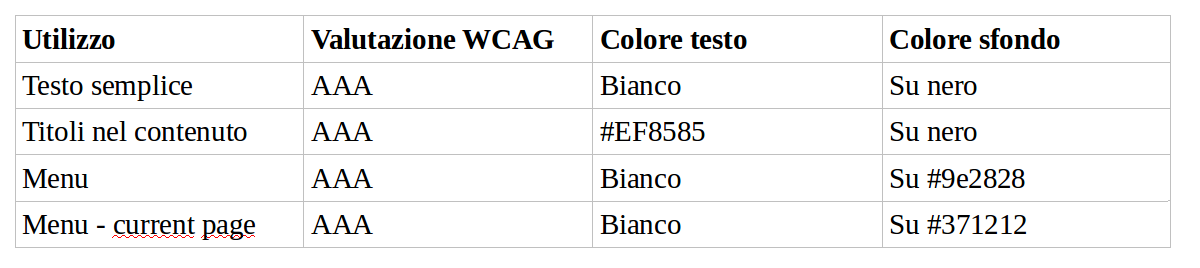
\includegraphics[scale=0.30]{colori_tabella.png}
% \caption{Valutazioni WCAG per i principali accoppiamenti di colore}
% \end{figure}
\begin{figure}[h]
\centering
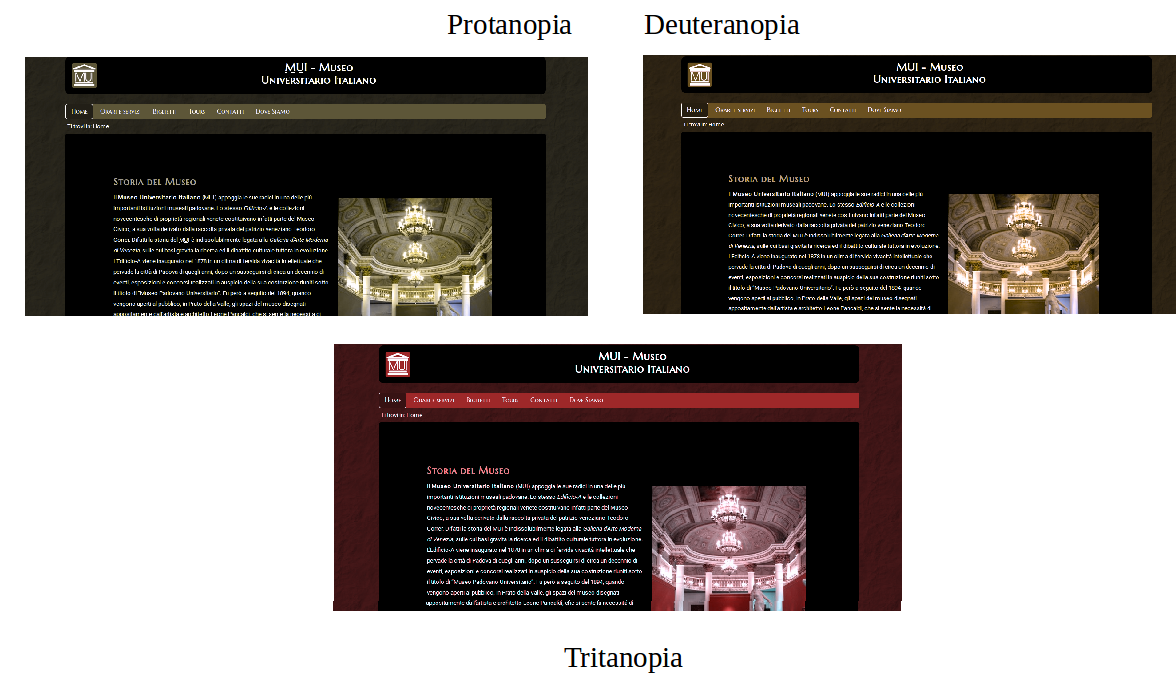
\includegraphics[scale=0.30]{daltonismo.png}
\caption{Vista della home page per chi soffre di daltonismo}
\end{figure}

\subsection{Testo}
Il testo viene presentato con una dimensione sufficiente ad una facile lettura anche per persone ipovedenti. Il Google font è stato scelto proprio in questa ottica. Per il testo semplice viene usato un font senza grazie che facilita la lettura. Oltre a questo la dimensione del carattere è stata impostata tramite “em”, in modo da adattare il testo in funzione delle caratteristiche preferite dall’utente.

\subsection{Immagini}
Sono presenti alcune immagini di contenuto nelle pagine. Non sono presenti immagini a scopo di presentazione o abbellimento, ad eccezione dello sfondo della pagina (pattern rosso scuro) che è stato inserito tramite CSS.
Per le immagini di contenuto, è stata fornita l'alternativa testuale all'immagine utilizzando il tag <img> con l'attributo alt, che descrive il contenuto dell'immagine in maniera concisa.
Anche per stabilire le dimensioni delle immagini sono state usate le percentuali o gli em.

\subsection{Tabelle}
Per rappresentare efficacemente i dati riguardanti i biglietti è stata utilizzata una tabella, che attraverso alcuni piccoli accorgimenti è stata resa accessibile.
I tag caption e summary permettono di rendere più accessibili le tabelle agli utenti non vedenti. E' stato utilizzato l’attributo scope si possono associare le intestazioni alle celle.
La tabella si vede correttamente anche da dispositivo mobile, come illustrato in figura.

\begin{figure}[h]
\centering
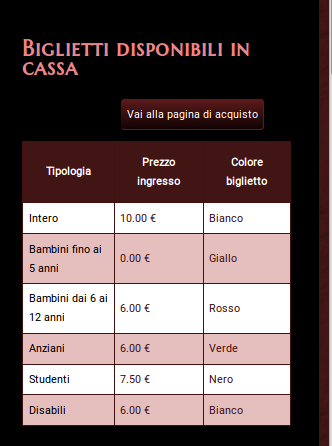
\includegraphics[scale=0.30]{vista_mobile_tabella.png}
\caption{Vista da smartphone della tabella}
\end{figure}

\subsection{Forms}
I campi dei form sono corredati con le apposite etichette (label) e le voci affini sono state raggruppate. In caso di errore l’utente viene informato in modo chiaro su quale sia l’errore e, se possibile, si è fatto in modo che l’utente non sia costretto a ripopolare tutti i campi. Per maggiori dettagli vedere le sezioni JavaScript e PHP

\subsection{Navigabilità}
La navigazione deve essere logica ed intuitiva, l’utente deve capire dove si trova, per evitare il disorientamento. A tal fine su tutte le pagine è presente la dicitura “Ti trovi in:”.\\
La destinazione di ciascun link è assolutamente chiara e inconfondibile, grazie a diciture significative ed autoesplicative.
Nelle pagine più lunghe è presente il collegamento che permette di tornare a inizio pagina in
modo tale da permettere una navigazione semplice e veloce.\\
Si è verificato che utilizzando il tasto tab l'utente riesca a spostarsi in maniera corretta da un link all'altro. Essendo il sito ben progettato, il percorso seguito dai tab index di default è appropriato, quindi non è stata necessaria la definizione di tab index speciali.\\
In caso di collegamenti rotti o altri problemi, l'utente viene reindirizzato presso la pagina "notfound.html", creata in linea con lo stile utilizzato nel resto del sito, per cercare di rendere questa esperienza meno negativa.

\subsection{Altri accorgimenti grafici}
Si è evitato di utilizzare oggetti in movimento o scritte lampeggianti, per non provocare disturbi a cui soffre di epilessia o disturbi della concentrazione.
Il testo, ad eccezione dei sottotitoli e delle immagini contenenti testo, può essere ridimensionato fino al 200 percento senza l'ausilio di tecnologie assistite e senza perdita di contenuto e funzionalità.
Le pagine sono state organizzate in modo che possano essere lette anche quando i fogli di stile siano disabilitati o non supportati.

\subsection{Altri accorgimenti di contenuto}
Le parole in inglese o francese (home, tour) sono state racchiuse dallo span lang.
Sono state utilizzate le espansioni per le abbreviazioni utilizzando il tag <abbr>.
Ci siamo assicurati che le pagine siano utilizzabili quando script, applet, o altri oggetti di programmazione sono disabilitati oppure non supportati.

\clearpage
\section{JavaScript}
Per la costruzione del sito ci è sembrato opportuno, in alcuni casi, fare uso di un linguaggio di programmazione lato client. Abbiamo optato nella scelta del Javascript per ovvie ragioni di popolarità. Tuttavia si è preferito limitarne l'uso, ove superfluo: scelta dettata dal non completo supporto da parte del pubblico a cui il nostro sito si rivolge. Detto ciò il sito rimane interamente utilizzabile anche in assenza di Javascript, e la sua eventuale disabilitazione da parte dell'utente, anche malevolo, non ne compromette le funzionalità.

\subsection{Pagina dove siamo}
Nella sezione "Dove siamo" il Javascript è stato adoperato per la visualizzazione interattiva della mappa di GoogleMaps; in caso di mancato supporto invece sarà visualizzata un'immagine raffigurante la piantina del luogo geografico degli edifici. Anche in questo caso la scelta di GoogleMaps, in luogo di altri servizi, magari più liberi, come OpenStreetMap è stata dettata dalla popolarità.

\subsection{Controlli nei form lato client}
Il Javascript assume anche un ruolo importante nella validazione dei campi dei form. Particolare attenzione è stata posta per i form dove un utente frettoloso potrebbe facilmente inserire stringhe erronee nei vari campi. Nel caso di sbaglio da parte dell'utente, un messaggio di errore compare a fianco o sotto i campi scorretti.

Laddove i controlli erano comunque necessari in PHP, abbiamo ritenuto importanti, in alcuni casi, ulteriori controlli Javascript, non ritenendoli codice ridondante bensì prevenzione di richieste inutili al server.

Per quanto riguarda gli utenti \textit{malevoli}, questi hanno chiaramente accesso alla parte client del sito, e potrebbero compromettere sia i form XHTML sia la parte Javascript. Tuttavia ogni tentativo erroneo o consapevolmente ostile fallisce grazie a una serie di controlli PHP intrapresi dal server che ne invaliderebbero le richieste.

\clearpage
\section{PHP}
\subsection{Considerazioni generali}
Le pagine consultabili dagli utenti non autenticati che hanno richiesto l'uso di PHP sono le pagine tours, biglietti e acquista biglietti. Queste pagine hanno infatti bisogno di interagire con il database per la visualizzazione e il salvataggio di dati. Oltre a questo è anche presente la pagina di accesso all'area di amministrazione.\\
Le pagine relative alla sezione di amministrazione sono tutte realizzate in PHP in quanto necessario, oltre che per l'accesso al database, anche per la gestione delle sessioni di login.\\
Dove necessario vengono usate le variabili di sessione del PHP per gestire messaggi di errore o di altro tipo da mostrare agli utenti in seguito alle operazioni eseguite. Tramite questa tecnica è possibile mostrare informazioni in maniera semplice e diretta, senza dover ricorrere a pagine di errore dedicate. Questo aumenta notevolmente la facilità d'uso del sito e migliora l'esperienza dell'utente al quale viene riproposta immediatamente la pagina che ha generato il messagio, permettendogli quindi di ripetere l'operazione. In caso di problemi nell'inserimento dei dati di un form vengono inoltre segnalati tutti gli errori.\\
Per cercare di rendere più modulare e manutenibile possibile il codice PHP si è deciso di utilizzare quanto più possibile le funzioni. Queste si dividono in due gruppi principali, le funzioni generiche per il recupero e la manipolazione delle informazioni salvate su database, presenti nel file functions.php e le funzioni per la stampa del codice HTML necessario alla creazione delle pagine, salvate nel file print\_functions.php. Così facendo le pagine PHP accessibili dal sito si riducono ad una serie di chiamate alle funzioni necessarie. Inoltre, con la divisione delle funzioni di stampa dalle altre, si è cercato di dividere la parte di contenuto da quella di comportamento.\\

\subsection{Sicurezza}
Per quanto riguarda la sicurezza viene eseguito un controllo sulla sessione per tutte le pagine di amministrazione, se tale controllo fallisce, ovvero se l'utente non risulta autenticato o se la sessione è scaduta, l'utente è reindirizzato verso la home page del sito. I dati salvati nelle variabili di sessione sono inoltre utilizzati per gestire le due diverse tipologie di utenti autenticati.\\
Per i file PHP contenenti le funzioni e i dati di accesso al database, che vengono inclusi quando necessario, viene invece eseguito un controllo su una variabile costante, se questi file vengono chiamati in maniera diretta, invece che da un altra pagina PHP in cui è definita la variabile necessaria, l'utente è rimandato alla pagina di errore 404 del sito.\\

\subsection{Controlli lato server}
Sono stati fatti dei controlli lato server per garantire il corretto inserimento degli input. Più nel dettaglio i principali controlli sono:
\begin{itemize}
\item Nomi e nominativi: questi campi accettano unicamente lettere, numeri e spazi, è possibile definire un minimo e un massimo numero di caratteri. Il controllo viene eseguito tramite un'espressione regolare;
\item Date: i dati inseriti sono verificati tramite la funzione \textit{checkdate} di PHP, nel caso i dati inseriti rappresentino una data valida questa viene restituita nel formato standard YYYY-MM-DD;
\item Numeri: a seconda del contesto è possibile che questi campi accettino numeri interi o decimali, in entrambi i casi è possibile definire il numero massimo di cifre da utilizzare (nel caso dei decimali solo per la parte intera), la validazione viene eseguita tramite un'espressione regolare.
\end{itemize}
L'inserimento di una data prevede anche controlli aggiuntivi per accertare che sia una data sensata nel suo contesto, non è possibile per esempio acquistare un biglietto per una data già passata o eseguire una ricerca tra due date non consecutive.\\
Tutti gli input vengono sottoposti alla funzione \textit{trim} in modo da eliminare eventuali spazi aggiuntivi in testa ed in coda. I campi di tipo testo (nominativi e descrizioni) vengono inoltre sottoposti alle funzioni \textit{stripslashes} e \textit{strip\_tags}, queste funzioni eliminano gli slash ed eventuali tag HTML, questo permette di garantire maggior sicurezza sui dati, in particolare verso l'inserimento di codice Javascript malevolo.\\
Non vengono eseguiti controlli lato server sui dati inseriti nel form di login in quanto viene fatto un controllo implicito quando i dati sono confrontati con quelli presenti nel database.

\subsection{Pagine PHP}
\subsubsection{Tours}
Nella pagina tours vengono mostrati i vari tour presenti nel database. Per ogni tour quindi si mostra il nome, la descrizione, il prezzo, e il nome della guida.

\subsubsection{Biglietti}
Nella pagina biglietti attraverso il linguaggio PHP vengono generate le righe della tabella. Ogni riga mostra una certa tipologia di biglietto presente nel database. Per ogni tipologia quindi si mostra la descrizione, il prezzo e il costo dell'audioguida.

\subsubsection{Acquista biglietti}
Nella pagina di acquista biglietti viene visualizzato un form per l'acquisto di biglietti. I dati da inserire sono un un nominativo, la data della visita, il tour che si desidera e il numero di biglietti richiesti per ogni tipologia. La parte di form con le tipologie di biglietti è creata in maniera dinamica tramite PHP.

\subsubsection{Pagina di accesso all'area di amministrazione}
La pagina visualizza un form in cui sono richiesti username e password per eseguire l'accesso all'area di amministrazione. Nel caso in cui un utente già autenticato visiti la pagina viene visualizzato un messaggio in cui si avvisa l'utente che è già autenticato e viene proposto il link per la home page dell'amministrazione. I controlli sono eseguiti utilizzando le sessioni gestite tramite codice PHP.

\subsection{Pagine di amministrazione}
\subsubsection{Home page amministrazione}
In questa pagina vengono proposti i link alle varie attività che può eseguire l'utente loggato. Nel caso questo sia una guida i link proposti saranno solo un sottoinsieme di quelli che vengono invece mostrati agli utenti di tipo segreteria. Il controllo sulla tipologia degli utenti viene fatto sfruttato le variabili di sessione del PHP all'interno delle quali vengono salvati i dati relativi all'utente loggato.

\subsubsection{Cerca e visualizza biglietti}
Da questa pagina, inserendo una data di inizio e una data di fine, viene generata la lista dei biglietti acquistati in quel periodo di tempo. Se non viene trovato nessun biglietto, se la data è inserita in un formato non corretto o se la data di inizio ricerca è successiva a quella di fine viene visualizzato un messaggio che informa l'utente.

\subsubsection{Modifica tour}
In questa pagina attraverso viene visualizzato un form con i dati relativi ad ogni tours presente nel database, questi dati possono essere modificati e salvati oppure, tramite una checkbox di conferma, il tour selezionato può essere eliminato. Se i dati inseriti non sono correti viene visualizzato un messaggio d'errore altrimenti viene informato l'utente che la modifica è stata eseguita con successo.

\subsubsection{Modifica tipologie dei biglietti}
Vengono visualizzati dei form per ogni tipologia di biglietto con i relativi dati, questi dati possono essere modificati e salvati. Se i dati inseriti non sono correti viene visualizzato un messaggio d'errore altrimenti viene informato l'utente che la modifica è stata eseguita con successo.
Questa pagina non è accessibile alle guide. L'accesso è controllato tramite le variabili di sessione, se una guida prova ad accedervi in maniera diretta viene visualizzato un avviso per informare l'utente che non ha accesso alla pagina e viene proposto il link alla home page di amministrazione.

\subsubsection{Inserisci tour}
La pagina presenta un form dove si possono inserire i dati relativi ad un nuovo tour. Se i dati inseriti non sono correti viene visualizzato un messaggio d'errore altrimenti viene informato l'utente che la modifica è stata eseguita con successo.
Questa pagina non è accessibile alle guide. L'accesso è controllato tramite le variabili di sessione, se una guida prova ad accedervi in maniera diretta viene visualizzato un avviso che per informare l'utente che non ha accesso alla pagine e viene proposto il link alla home page di amministrazione.

\subsection{Altri script PHP}
Oltre alle pagine accessibili dal sito ci sono una serie di altri file PHP che vengono utilizzati, nello specifico:
\begin{itemize}
    \item i file contenenti le funzioni necessarie che vengono inclusi quando necessario;
    \item gli script utilizzati dai form che eseguono il controllo dei dati e la gestione di eventuali errori.
\end{itemize}
\clearpage
\section{Tecnologie e strumenti utilizzati}

\subsection{Installazione del sito}
Non è necessaria alcuna operazione particolare per l'installazione del sito, ma bisogna assicurarsi di caricare il file nascosto \textit{.htaccess} per visualizzare correttamente la pagina 404.

\subsection{Tecnologie utilizzate}
Seguendo le regole progettuali del Corso di Tecnologie Web sono state utilizzate le seguenti tecnologie: \begin{itemize}
\item XHTML 1.0 Strict per la struttura del contenuto
\item CSS versione CSS 2 e qualche proprietà del CSS 3
\item JAVASCRIPT per la gestione di alcune peculiarità lato client
\item PHP come linguaggio di programmazione lato server
\end{itemize}

\subsection{Strumenti di validazione}
Gli strumenti di validazione utilizzati sono:
\begin{itemize}
\item Validazione HTML: https://validator.w3.org/
\item Validazione CSS: https://jigsaw.w3.org/css-validator/
\item Test contrasto: http://contrastchecker.com/
\item Test daltonismo: http://www.color-blindness.com/coblis-color-blindness-simulator/
\end{itemize}

\subsection{Test su diversi browser}
Il sito è stato testato su:
\begin{itemize}
\item Firefox 50
\item Internet Explorer 11
\item Internet Explorer 8
\item Google Chrome 56
\item Safari
\item Opera
\end{itemize}
Tutte le pagine si vedono correttamente, persino sulla più vecchia versione di Internet Explorer 8. A titolo esemplificativo si riporta la visualizzazione della pagina biglietti sui vari browser.

\begin{figure}[H]
    \centering
    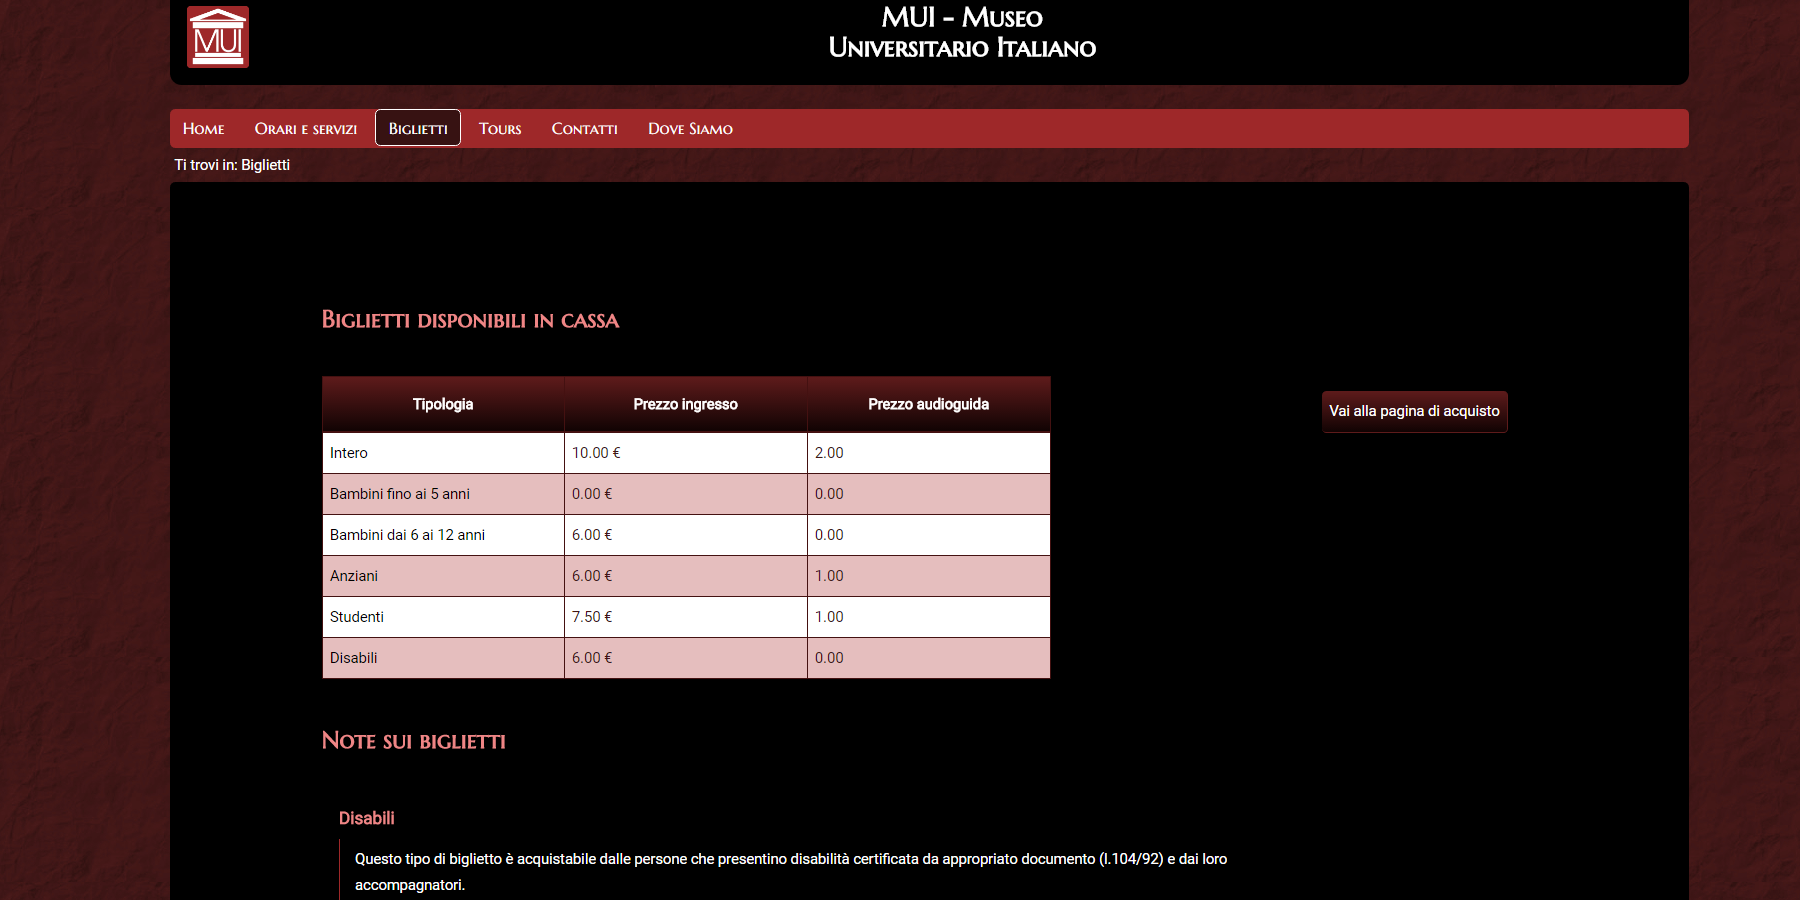
\includegraphics[scale=0.10]{biglietti_chrome.png}
    \caption{Vista da Google Chrome della pagina biglietti}
\end{figure}

\begin{figure}[H]
    \centering
    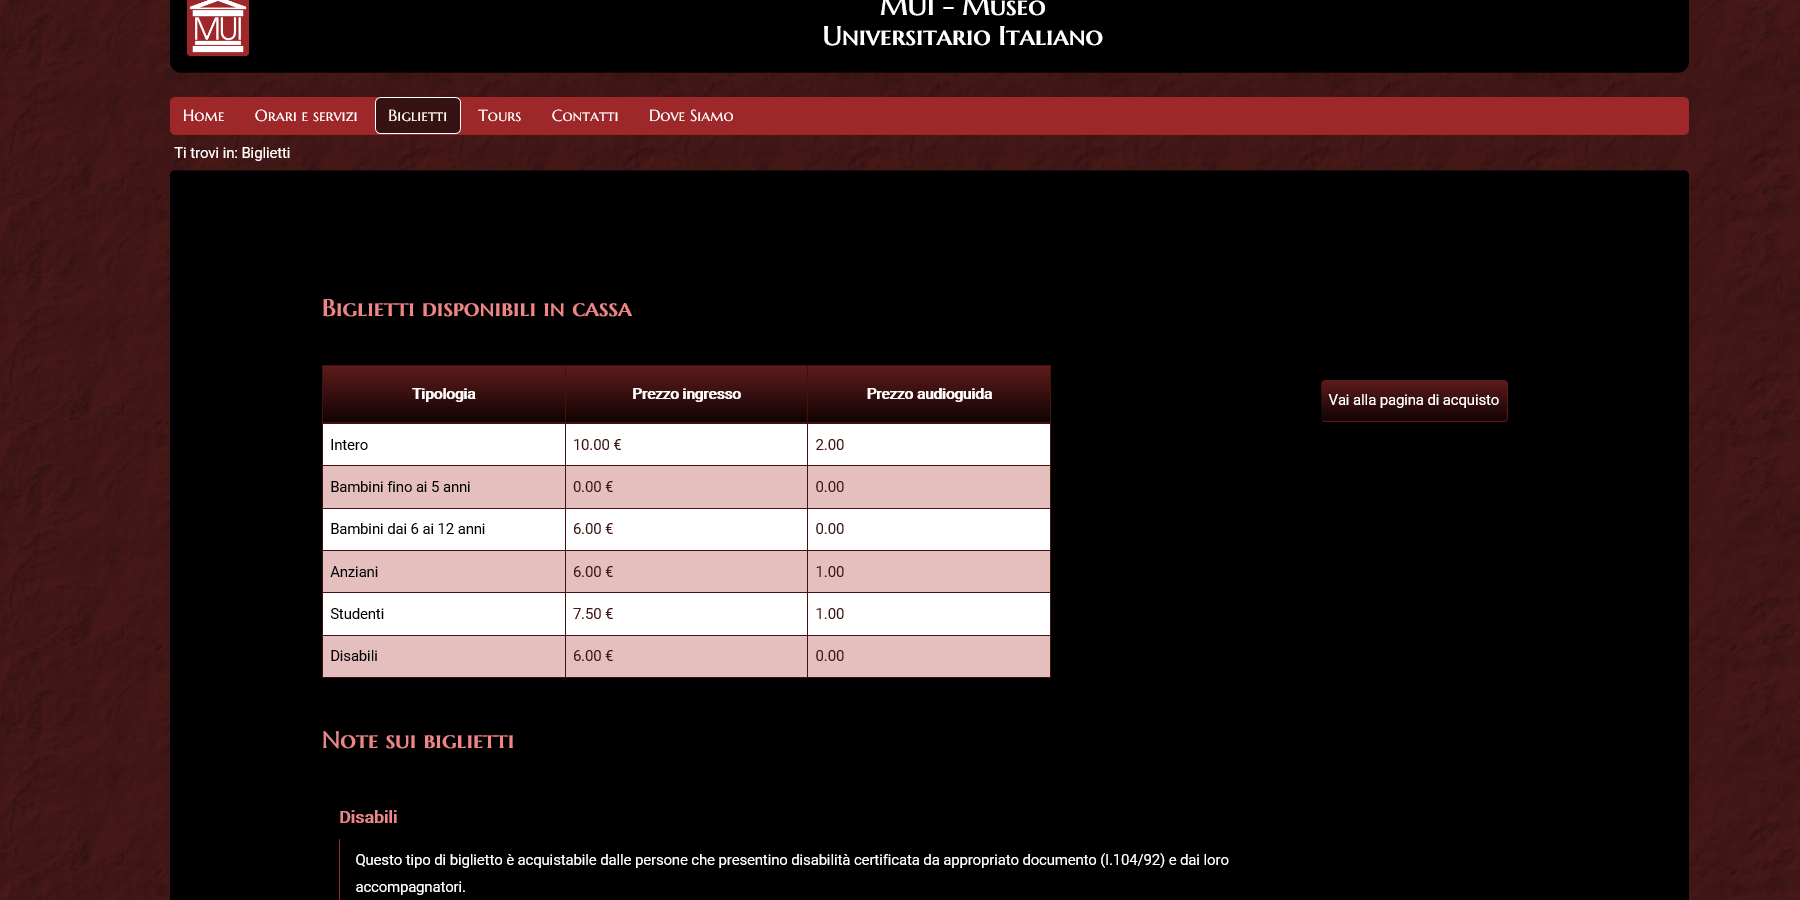
\includegraphics[scale=0.10]{biglietti_explorer11.png}
    \caption{Vista da Internet Explorer 11 della pagina biglietti}
\end{figure}

\begin{figure}[H]
    \centering
    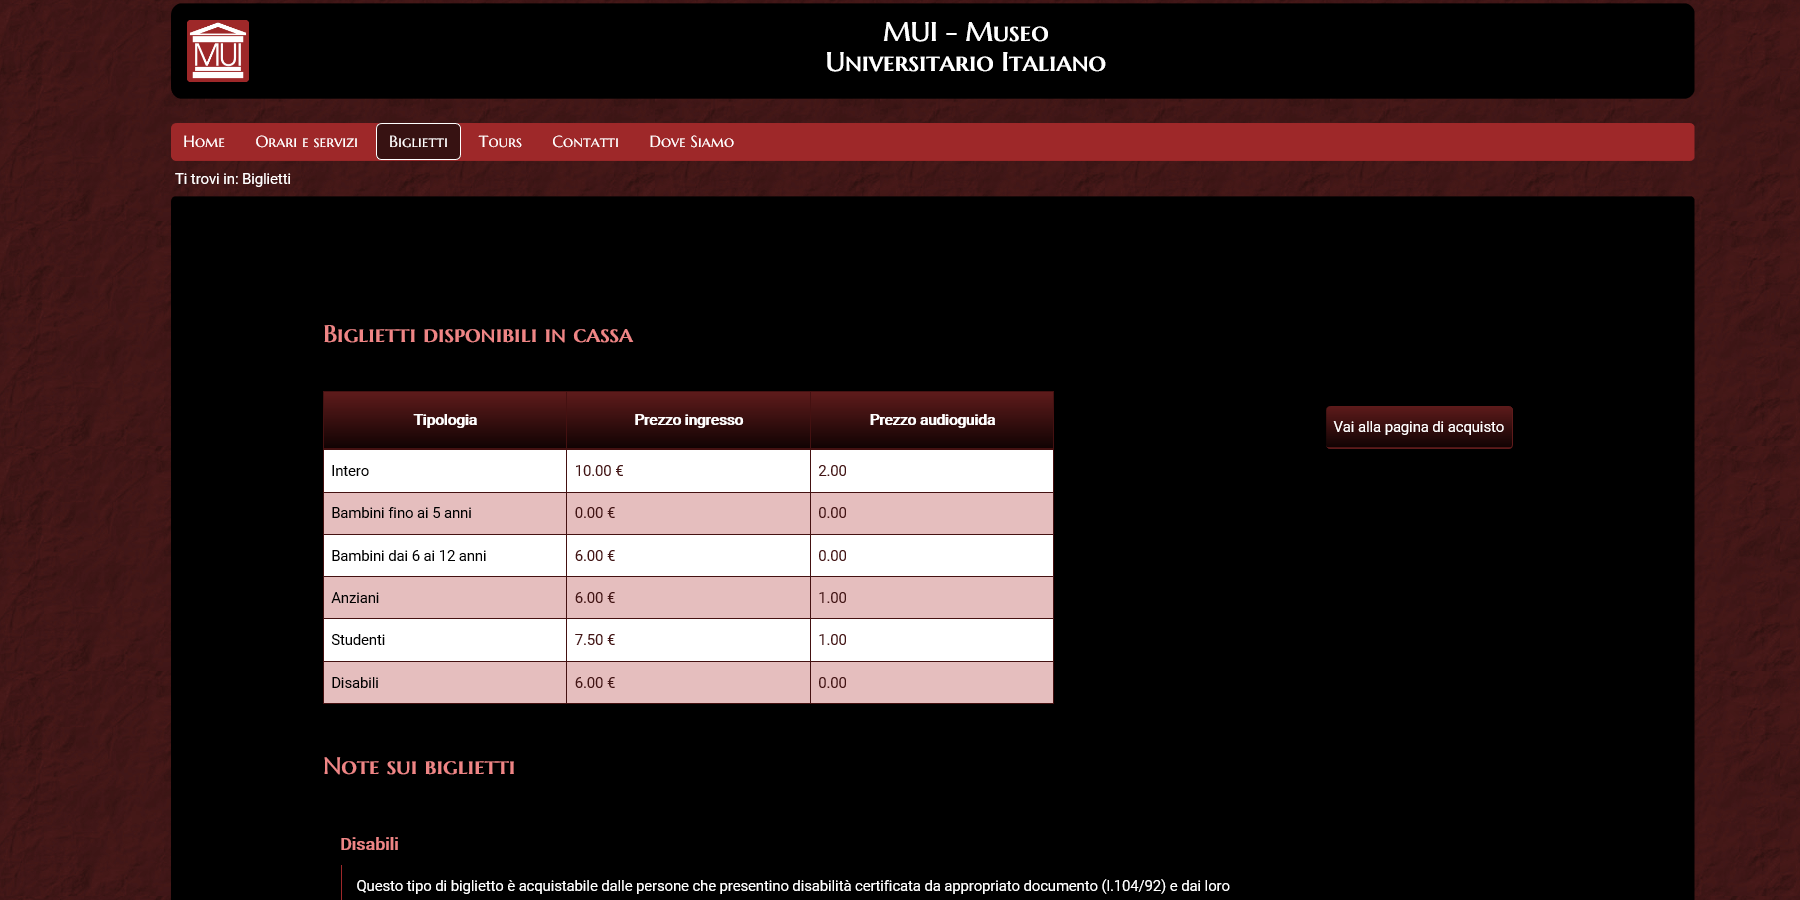
\includegraphics[scale=0.10]{biglietti_explorer8.png}
    \caption{Vista da Internet Explorer 8 della pagina biglietti}
\end{figure}

\begin{figure}[H]
    \centering
    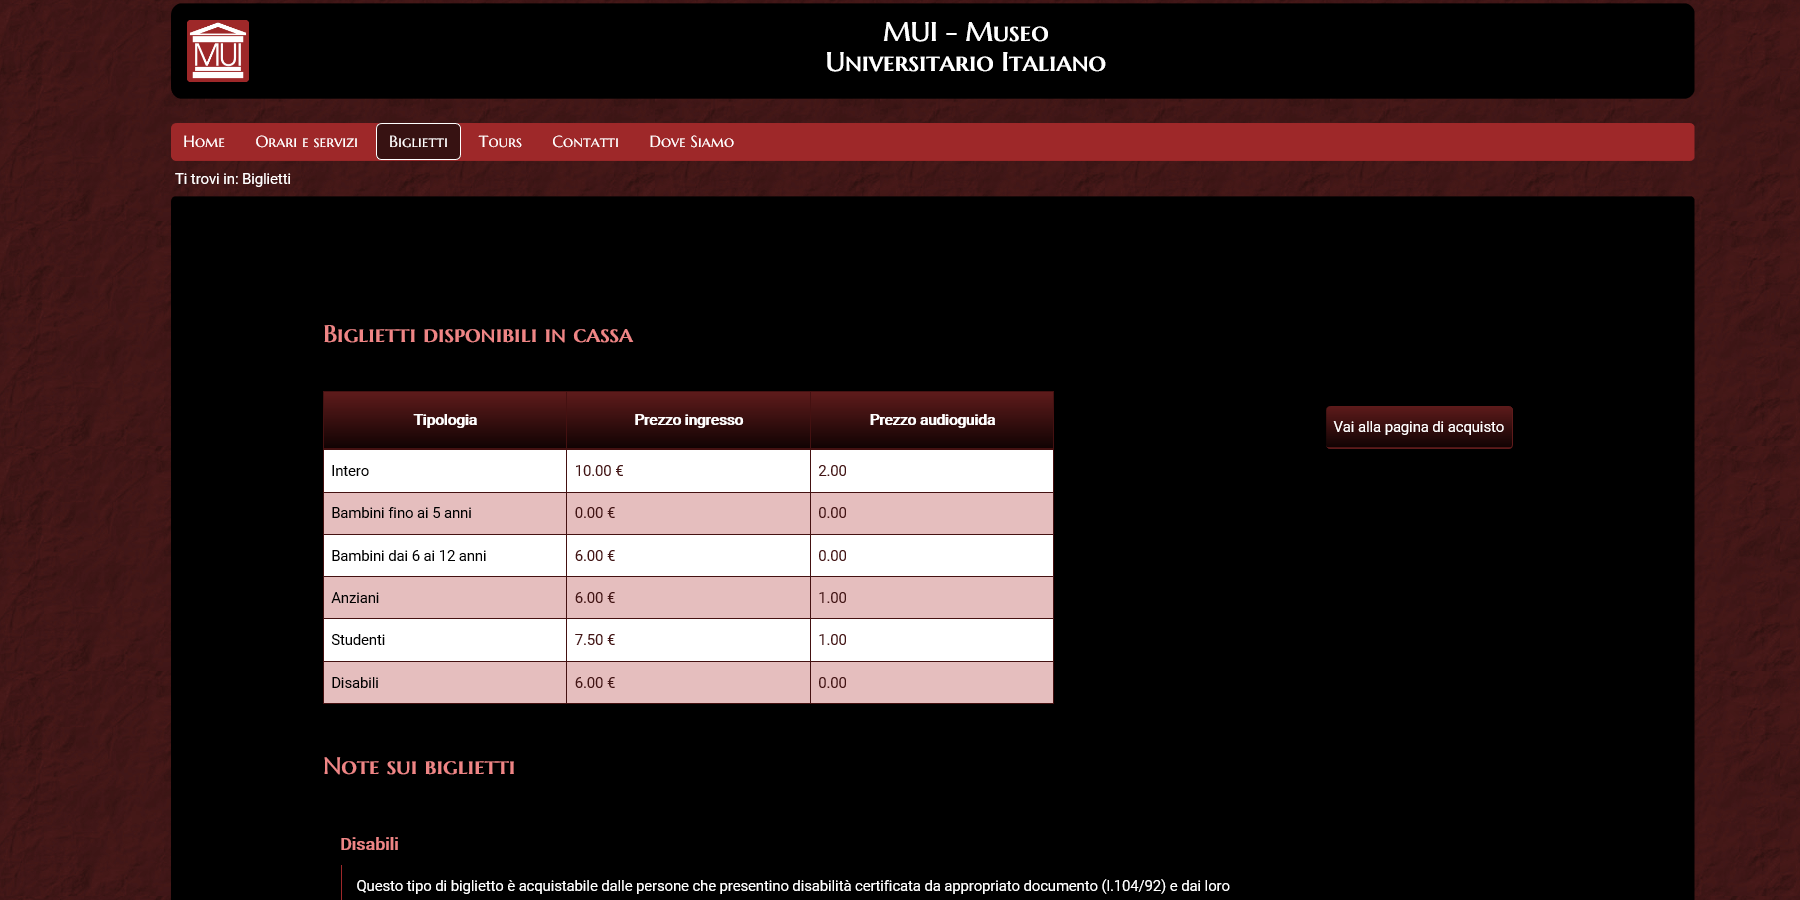
\includegraphics[scale=0.10]{biglietti_firefox.png}
    \caption{Vista da Mozilla Firefox della pagina biglietti}
\end{figure}

\begin{figure}[H]
    \centering
    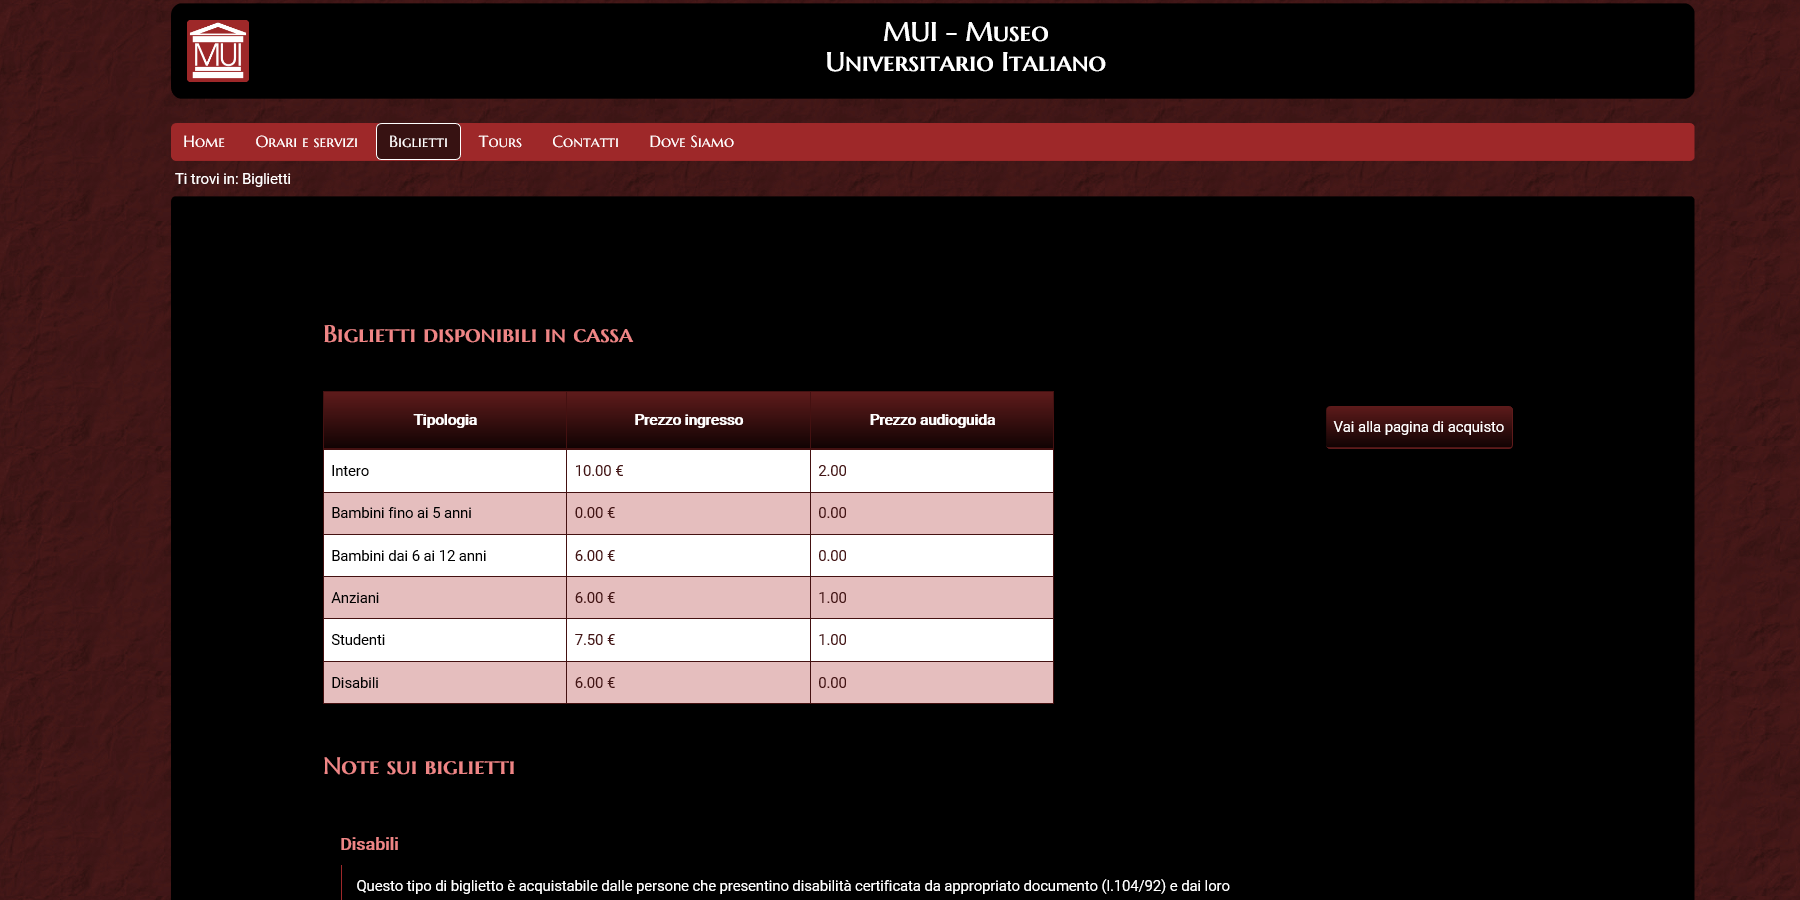
\includegraphics[scale=0.10]{biglietti_opera.png}
    \caption{Vista da Opera della pagina biglietti}
\end{figure}

\begin{figure}[H]
    \centering
    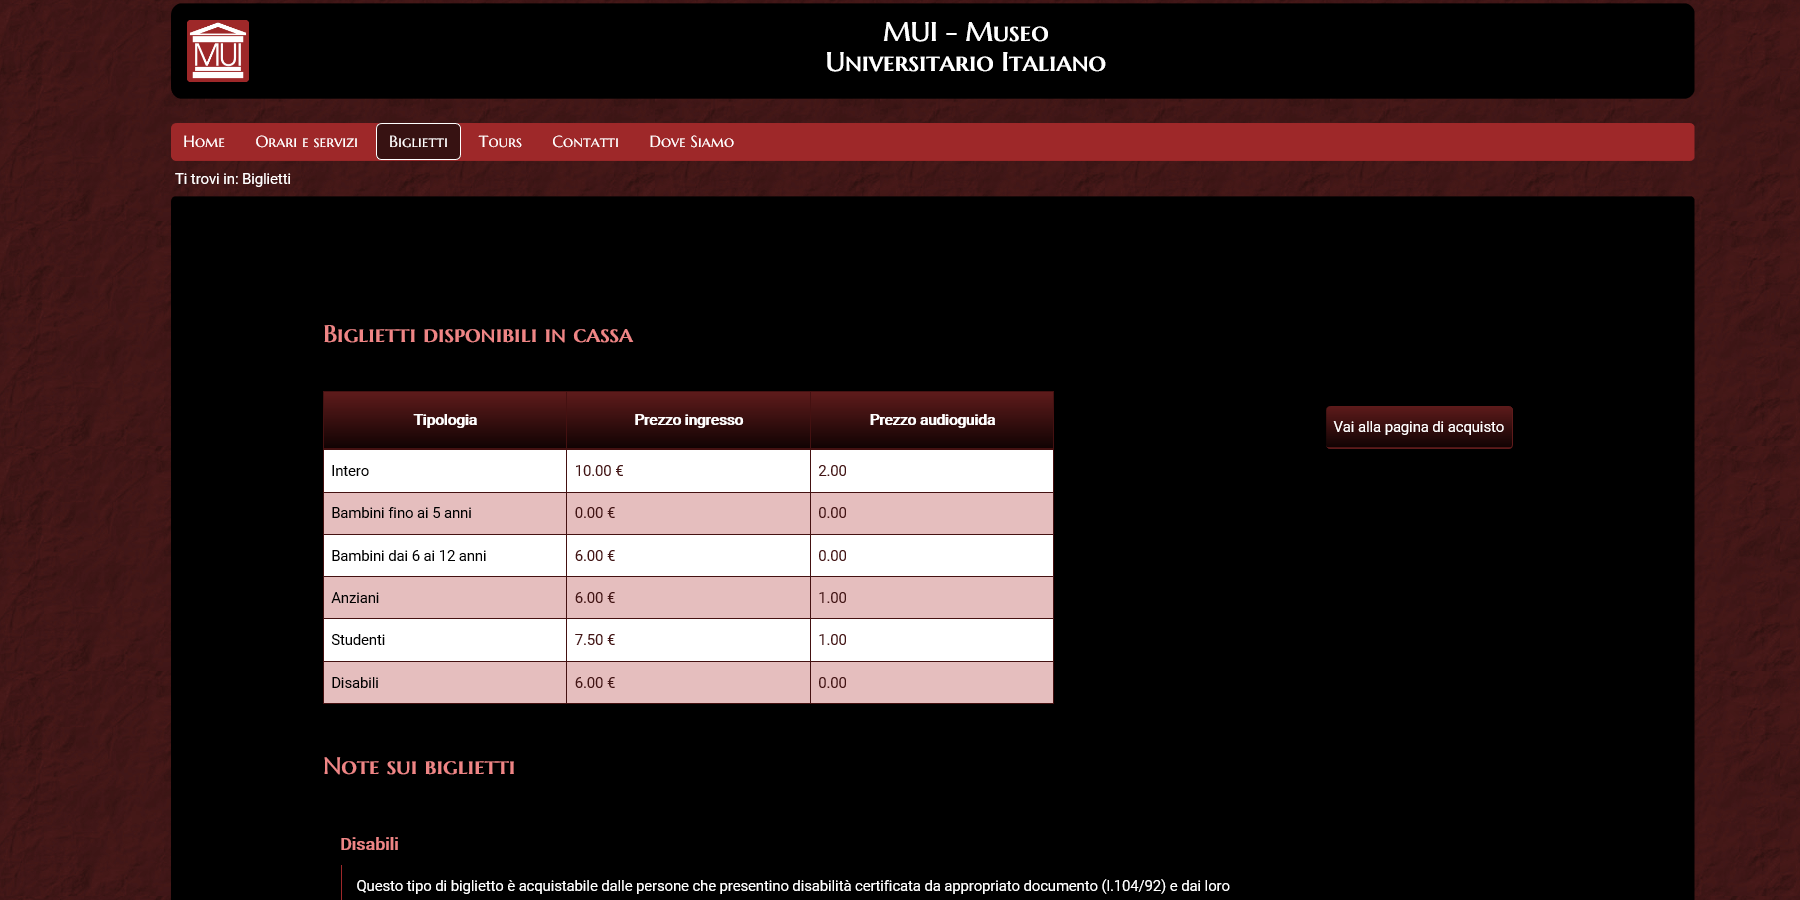
\includegraphics[scale=0.10]{biglietti_safari.png}
    \caption{Vista da Safari della pagina biglietti}
\end{figure}

\clearpage
\subsection{Strumenti ausiliari}
Per la condivisione e il verionamento del codice è stato usato git e in particolare il servizio offerto da GitHub.\\
Per il coordinamento e la comunicazione interna è stato usato Telegram.\\
Per la relazione è stato utilizzato TexStudio.

\subsection{Metodologia di lavoro}
Per lo sviluppo del progetto c’è stato un continuo coinvolgimento di tutti, anche se alcuni membri hanno dedicato più attenzione ad alcuni aspetti rispetto che ad altri, secondo le proprie inclinazioni e le proprie abilità. Più nel dettaglio:
\begin{itemize}
 \item Meneguzzo Silvio: HTML, SQL, relazione
 \item Petenazzi Giulia: CSS, PHP, relazione
 \item Prete Giovanni: PHP, SQL
 \item Vianello Fabio: JavaScript, CSS
\end{itemize}

\end{document}
